% Options for packages loaded elsewhere
\PassOptionsToPackage{unicode}{hyperref}
\PassOptionsToPackage{hyphens}{url}
\PassOptionsToPackage{dvipsnames,svgnames,x11names}{xcolor}
%
\documentclass[
  11pt,
]{article}
\usepackage{amsmath,amssymb}
\usepackage{lmodern}
\usepackage{iftex}
\ifPDFTeX
  \usepackage[T1]{fontenc}
  \usepackage[utf8]{inputenc}
  \usepackage{textcomp} % provide euro and other symbols
\else % if luatex or xetex
  \usepackage{unicode-math}
  \defaultfontfeatures{Scale=MatchLowercase}
  \defaultfontfeatures[\rmfamily]{Ligatures=TeX,Scale=1}
  \setmainfont[]{Roboto}
  \setsansfont[]{Roboto}
\fi
% Use upquote if available, for straight quotes in verbatim environments
\IfFileExists{upquote.sty}{\usepackage{upquote}}{}
\IfFileExists{microtype.sty}{% use microtype if available
  \usepackage[]{microtype}
  \UseMicrotypeSet[protrusion]{basicmath} % disable protrusion for tt fonts
}{}
\makeatletter
\@ifundefined{KOMAClassName}{% if non-KOMA class
  \IfFileExists{parskip.sty}{%
    \usepackage{parskip}
  }{% else
    \setlength{\parindent}{0pt}
    \setlength{\parskip}{6pt plus 2pt minus 1pt}}
}{% if KOMA class
  \KOMAoptions{parskip=half}}
\makeatother
\usepackage{xcolor}
\IfFileExists{xurl.sty}{\usepackage{xurl}}{} % add URL line breaks if available
\IfFileExists{bookmark.sty}{\usepackage{bookmark}}{\usepackage{hyperref}}
\hypersetup{
  pdftitle={Democratic Spaces 2022},
  pdfauthor={Andreas Beger (Basil Analytics)},
  colorlinks=true,
  linkcolor={Maroon},
  filecolor={Maroon},
  citecolor={Blue},
  urlcolor={Blue},
  pdfcreator={LaTeX via pandoc}}
\urlstyle{same} % disable monospaced font for URLs
\usepackage[margin=1in]{geometry}
\usepackage{graphicx}
\makeatletter
\def\maxwidth{\ifdim\Gin@nat@width>\linewidth\linewidth\else\Gin@nat@width\fi}
\def\maxheight{\ifdim\Gin@nat@height>\textheight\textheight\else\Gin@nat@height\fi}
\makeatother
% Scale images if necessary, so that they will not overflow the page
% margins by default, and it is still possible to overwrite the defaults
% using explicit options in \includegraphics[width, height, ...]{}
\setkeys{Gin}{width=\maxwidth,height=\maxheight,keepaspectratio}
% Set default figure placement to htbp
\makeatletter
\def\fps@figure{htbp}
\makeatother
\setlength{\emergencystretch}{3em} % prevent overfull lines
\providecommand{\tightlist}{%
  \setlength{\itemsep}{0pt}\setlength{\parskip}{0pt}}
\setcounter{secnumdepth}{-\maxdimen} % remove section numbering
\newlength{\cslhangindent}
\setlength{\cslhangindent}{1.5em}
\newlength{\csllabelwidth}
\setlength{\csllabelwidth}{3em}
\newlength{\cslentryspacingunit} % times entry-spacing
\setlength{\cslentryspacingunit}{\parskip}
\newenvironment{CSLReferences}[2] % #1 hanging-ident, #2 entry spacing
 {% don't indent paragraphs
  \setlength{\parindent}{0pt}
  % turn on hanging indent if param 1 is 1
  \ifodd #1
  \let\oldpar\par
  \def\par{\hangindent=\cslhangindent\oldpar}
  \fi
  % set entry spacing
  \setlength{\parskip}{#2\cslentryspacingunit}
 }%
 {}
\usepackage{calc}
\newcommand{\CSLBlock}[1]{#1\hfill\break}
\newcommand{\CSLLeftMargin}[1]{\parbox[t]{\csllabelwidth}{#1}}
\newcommand{\CSLRightInline}[1]{\parbox[t]{\linewidth - \csllabelwidth}{#1}\break}
\newcommand{\CSLIndent}[1]{\hspace{\cslhangindent}#1}
\usepackage[labelfont=bf]{caption}
\usepackage{booktabs}
\usepackage{longtable}
\usepackage{array}
\usepackage{multirow}
\usepackage{wrapfig}
\usepackage{float}
\usepackage{colortbl}
\usepackage{pdflscape}
\usepackage{tabu}
\usepackage{threeparttable}
\usepackage{threeparttablex}
\usepackage[normalem]{ulem}
\usepackage{makecell}
\usepackage{xcolor}
\ifLuaTeX
  \usepackage{selnolig}  % disable illegal ligatures
\fi

\title{Democratic Spaces 2022}
\usepackage{etoolbox}
\makeatletter
\providecommand{\subtitle}[1]{% add subtitle to \maketitle
  \apptocmd{\@title}{\par {\large #1 \par}}{}{}
}
\makeatother
\subtitle{Updated forecasts and a refinement in how opening and closing
events are measured}
\author{Andreas Beger (Basil Analytics)\footnote{Email:
  \href{mailto:andy@basilanalytics.com}{\nolinkurl{andy@basilanalytics.com}}}}
\date{26 May 2022}

\begin{document}
\maketitle

{
\hypersetup{linkcolor=}
\setcounter{tocdepth}{2}
\tableofcontents
}
\hypertarget{summary}{%
\section{Summary}\label{summary}}

\begin{itemize}
\tightlist
\item
  The way that opening and closing events in the six spaces has changed.
  The new method (``ERT-lite'') is able to identify more gradual changes
  in the spaces that over the span of two or more years result in
  significant shifts. The old method was limited to identifying large
  single-year shifts--which are still included in the new method as
  well. This allows DemSpaces to, for example, pick up the more gradual
  closings in some of the spaces for Poland and Hungary over the
  2010s.\\
\item
  The new forecasts overall indicate higher risks of continued closing
  events, reflecting the ongoing global worsening of democratic
  governance. While on balance the trend leans towards negative, there
  are also still significant potentials for opening movements in other
  countries and spaces.
\item
  The accuracy of the v10 forecasts, which can now be fully assessed, is
  in line with the previous v9 accuracy. With AUC-ROC values of 0.7 the
  forecasts could be more accurate--0.8 or slightly higher is common in
  many political instability applications--but are informative additions
  over a naive baseline estimate. There is some indication that the
  stability of the most recent V-Dem version has increased, which would
  alleviate the shifting-ground problem induced by changes in historical
  data as each V-Dem version continues to refine the data.
\end{itemize}

(Note: the forecasts are indexed with the V-Dem data version used to
produce them. For the latest, v12 forecasts, I use ``v12'' to denote
forecasts using the old outcome coding method, and ``v12.1'' for the new
ERT-lite outcome coding method. Both sets of forecasts can be found in
the project repo
\href{https://github.com/vdeminstitute/demspaces/tree/main/archive}{demspaces/archive}
folder, but only the ``v12.1'' forecasts are shown in the dashboard.)

\hypertarget{ert-lite-new-method-for-identifying-opening-and-closing-events}{%
\section{ERT-lite: new method for identifying opening and closing
events}\label{ert-lite-new-method-for-identifying-opening-and-closing-events}}

Opening and closing events in the democratic spaces have so far been
based on large \emph{single}-year changes. However, sometimes there are
cases where the space in a country changes gradually but significantly
over a span of multiple years, without ever experiencing a large
single-year change that our coding approach to date would have
identified. Figure \ref{fig:poland-old} shows the governing space in
Poland. Since 2014 it has been experiencing gradual but steady declines.
With the old outcome coding method, none of those years were identified
as closing events.

\begin{figure}
\centering
\caption{Poland governing space: there is a large, gradual decrease since 2014, but no closing event is coded in the old method.\label{fig:poland-old}}
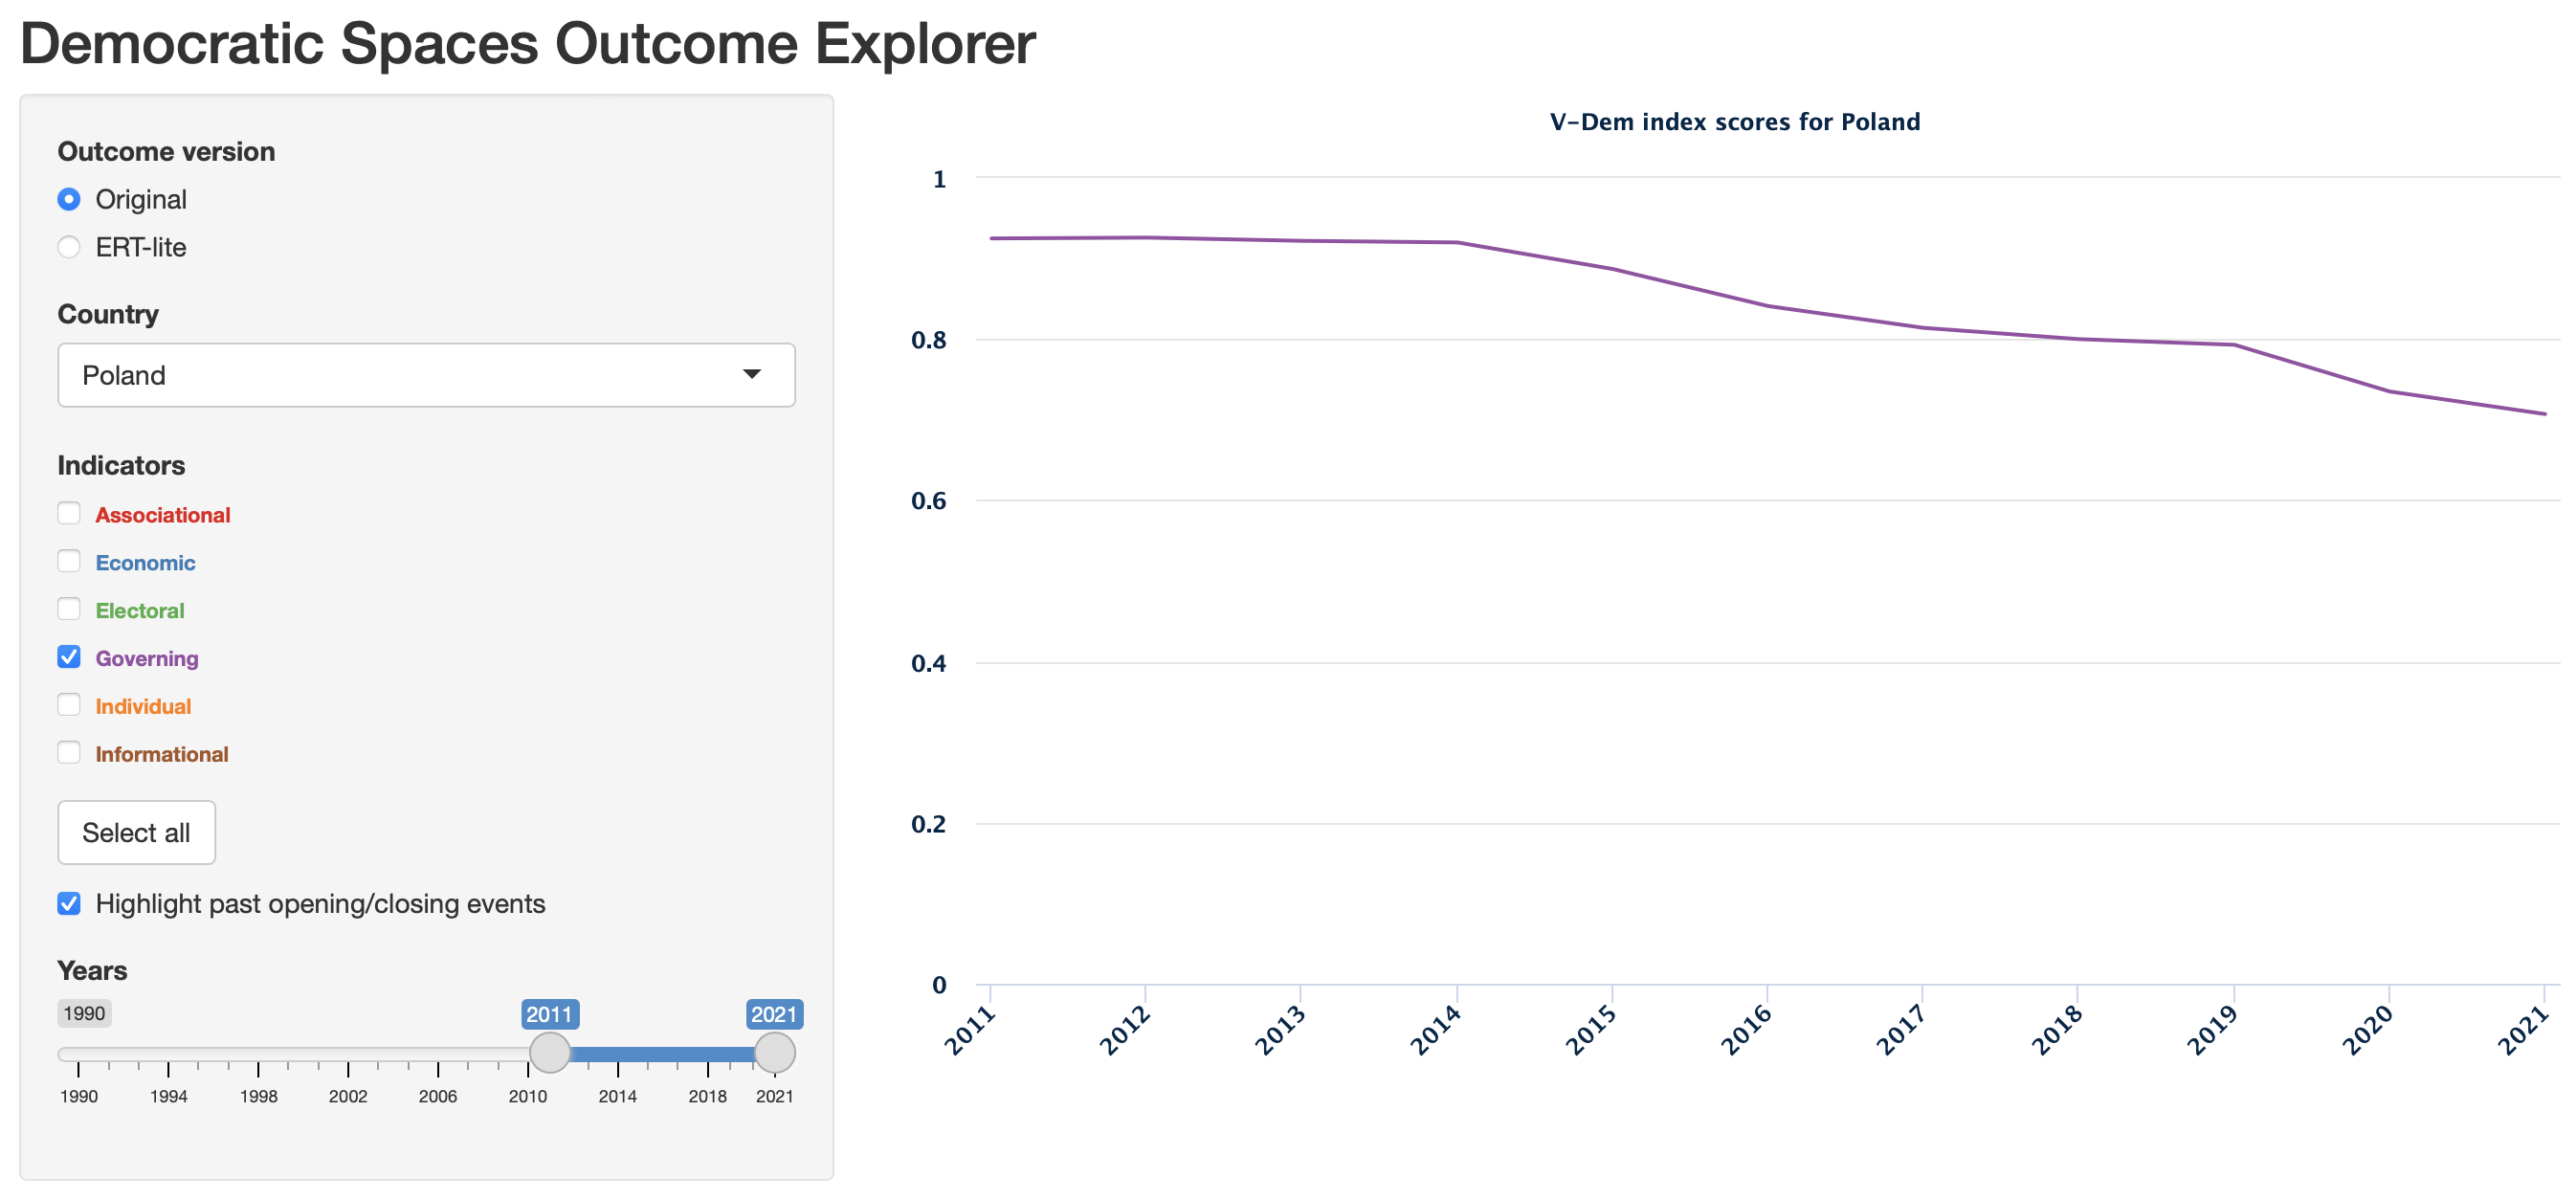
\includegraphics{report-figures/poland-governing.png}
\end{figure}

As part of the spring 2022 update, I investigated alternative outcome
coding methods that would better capture gradual transitions like this.
The end result, for the Poland governing case, is that most of the years
during the gradual transition since 2014 are now coded as such, as shown
in Figure \ref{fig:poland-new}.

\begin{figure}
\centering
\caption{Poland governing space with the new outcome coding method: most of the years during the gradual closing since 2014 are identified as closing events.\label{fig:poland-new}}
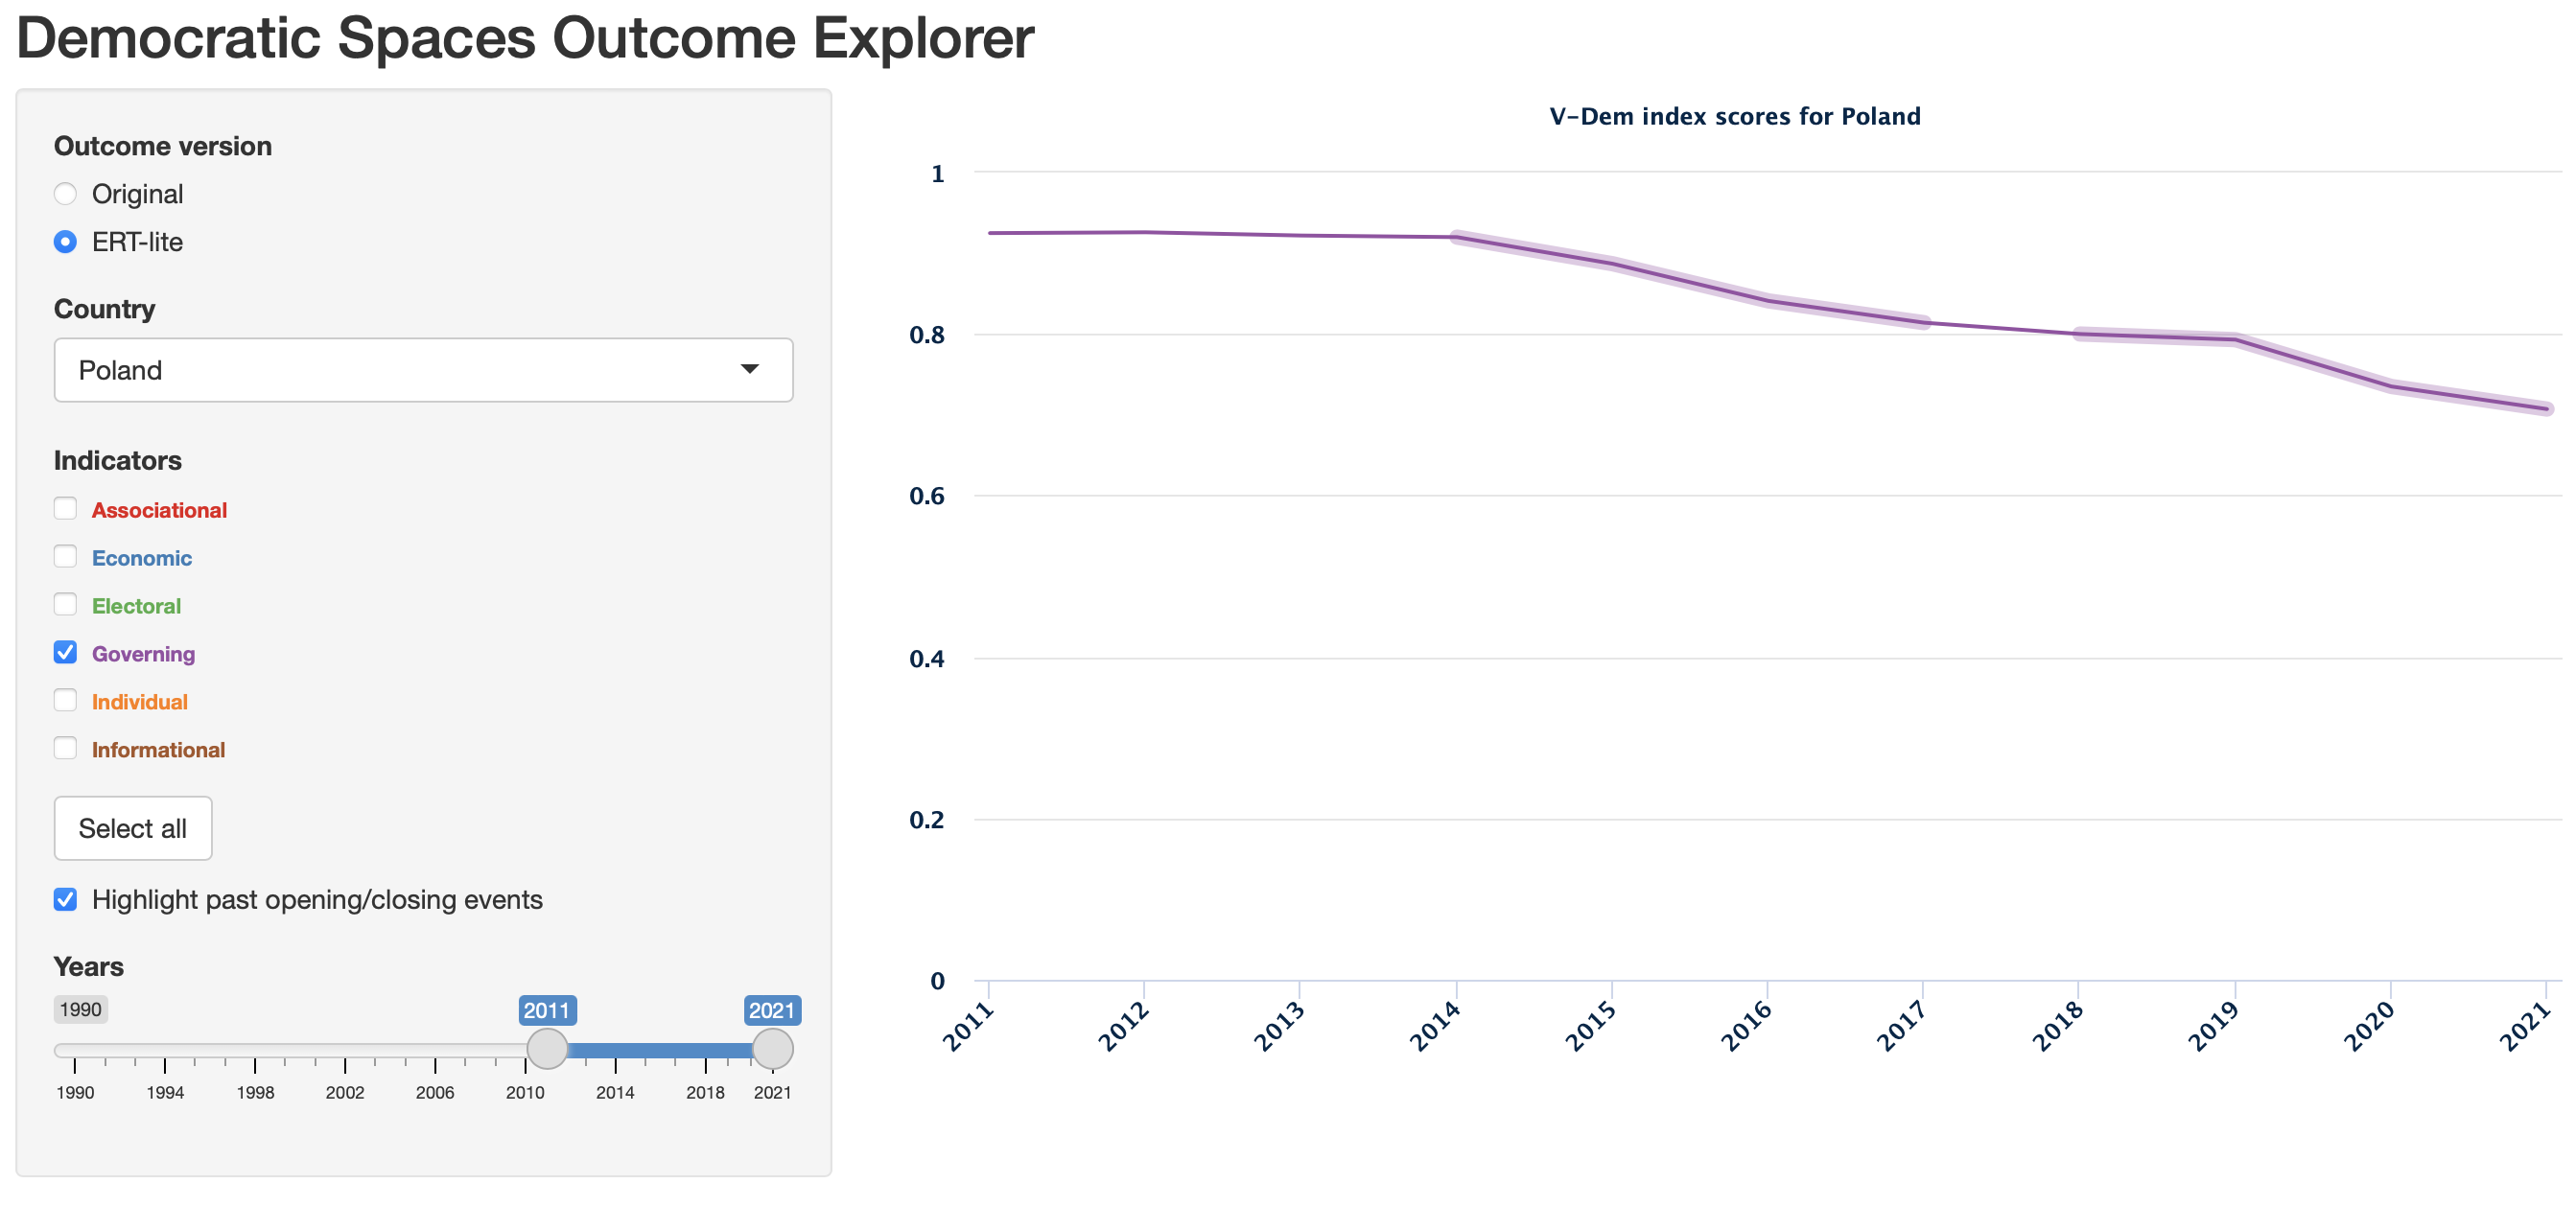
\includegraphics{report-figures/poland-governing-new.png}
\end{figure}

The new method for coding opening and closing events was inspired by
V-Dem's Episodes of Regime Transition project (Maerz et al. 2021), which
unifies autocratization and democratization in a single conceptual
framework (the eponymous ``episodes of regime transformations'') and
describes an algorithm for identifying relevant cases in the V-Dem
electoral democracy index. Their project and algorithm are much broader
in scope than what is required for democratic spaces, but it spurred the
improvement in the opening and closing cases coding method that I showed
above.

Namely, to date opening and closing events are coded if the change in a
space from the previous year exceeds a space-specific threshold value.
Each space has a different threshold because some spaces are in general
more fluctuating than others. To this single-year rule I added another
two-year rule: if the cumulative 2-year change in a space exceeds the
space threshold, \emph{and} each year's change from the previous year
exceeds 1/10th of the threshold (in the same direction), then both years
are coded as an being opening or closing events, depending on the
direction of change.

This is a minimally intrusive extension--we go from only considering a
single-year change to considering a two-year change--but manages to
capture gradual transitions better than the existing approach. Table
\ref{tab:outcome-comparison} shows the overall change in the number of
opening and closing events for 2021. In all but one instance--Electoral
openings--the number of events increases.

\begin{table}

\caption{\label{tab:outcome-comparison}Comparison of old- and new-style outcomes}
\centering
\begin{tabular}[t]{lrrrrrr}
\toprule
\multicolumn{1}{c}{} & \multicolumn{2}{c}{Closing} & \multicolumn{2}{c}{Same} & \multicolumn{2}{c}{Opening} \\
\cmidrule(l{3pt}r{3pt}){2-3} \cmidrule(l{3pt}r{3pt}){4-5} \cmidrule(l{3pt}r{3pt}){6-7}
Space & v12 & v12.1 & v12 & v12.1 & v12 & v12.1\\
\midrule
Associational & 20 & 28 & 135 & 123 & 14 & 18\\
Economic & 21 & 26 & 128 & 120 & 20 & 23\\
Electoral & 7 & 9 & 156 & 154 & 6 & 6\\
Governing & 18 & 28 & 143 & 129 & 8 & 12\\
Individual & 14 & 26 & 146 & 127 & 9 & 16\\
Informational & 20 & 30 & 143 & 125 & 6 & 14\\
\bottomrule
\end{tabular}
\end{table}

More details of this change are discussed in Section
``\hyperlink{ert-lite-assessment}{ERT-lite Assessment}'' below.

\hypertarget{overview-of-the-new-2022-2023-forecasts}{%
\section{Overview of the new 2022-2023
forecasts}\label{overview-of-the-new-2022-2023-forecasts}}

Because the new, ERT-style outcome coding method identifies more opening
and closing events than the old method, we should expect that the
forecasts generally are higher. But there may at the same time also be
systemic changes in the global risk of opening and closing events,
e.g.~increasing instability.

To untangle this, Figure \ref{fig:new-forecast-plot} summarizes last
year's ``v11'' forecasts, the directly comparable new ``v12'' forecasts
using the old-style outcome coding method, and the new ERT-lite
``v12.1'' forecasts. The only difference between the ``v12'' and
``v12.1'' forecasts is that the latter uses the new ERT-lite outcome
coding method. We can see that the forecasts in general are indeed
higher--from an average of 14.0\% to 19.4\% and 13.8\% to 18.5\% for
closing and opening, respectively. By comparing the ``v12'' and ``v11''
forecasts, where the only difference is that the former is using updated
data, we can assess whether there are global trends in the democratic
spaces. There are no dramatic changes. The average opening risk is
unchanged at 13.8\% and the average closing risk slightly increases from
13.4\% to 14.0\%.

\begin{figure}
\centering
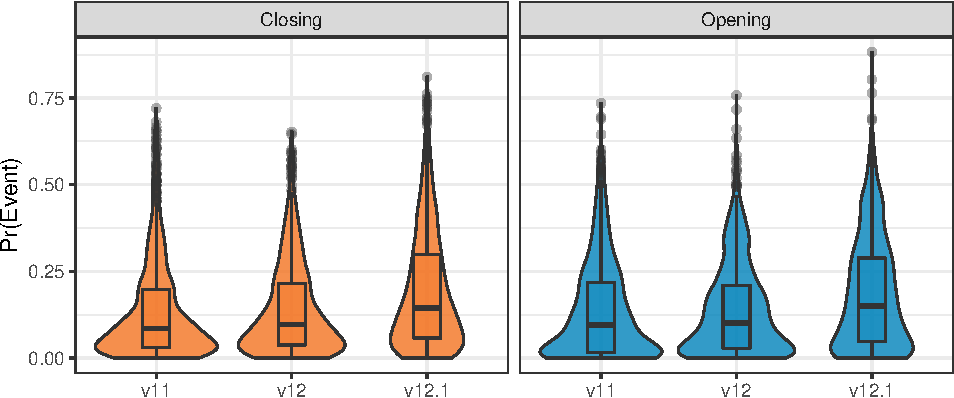
\includegraphics{democratic-spaces-2022_files/figure-latex/new-forecast-plot-1.pdf}
\caption{Distribution of last year's and this year's forecasts, pooled
over spaces.\label{fig:new-forecast-plot}}
\end{figure}

Table \ref{tab:topN} shows the 5 highest forecasts for opening and
closing changes for each of the 6 spaces (using the ``v12.1''
forecasts).

\begin{table}

\caption{\label{tab:topN}Highest risk for opening and closing events in each space.}
\centering
\begin{tabular}[t]{>{\raggedright\arraybackslash}p{12em}r>{\raggedright\arraybackslash}p{10em}r}
\toprule
\multicolumn{2}{c}{Closing} & \multicolumn{2}{c}{Opening} \\
\cmidrule(l{3pt}r{3pt}){1-2} \cmidrule(l{3pt}r{3pt}){3-4}
Country & Pr. & Country & Pr.\\
\midrule
\addlinespace[0.3em]
\multicolumn{4}{l}{\textbf{Associational}}\\
\hspace{1em}India & 0.74 & Bangladesh & 0.69\\
\hspace{1em}Philippines & 0.73 & Somalia & 0.65\\
\hspace{1em}Hungary & 0.69 & Pakistan & 0.58\\
\hspace{1em}Somalia & 0.64 & Nicaragua & 0.57\\
\hspace{1em}Thailand & 0.63 & South Korea & 0.52\\
\addlinespace[0.3em]
\multicolumn{4}{l}{\textbf{Economic}}\\
\hspace{1em}Brazil & 0.68 & Saudi Arabia & 0.88\\
\hspace{1em}Indonesia & 0.60 & China & 0.76\\
\hspace{1em}Colombia & 0.60 & Gabon & 0.64\\
\hspace{1em}India & 0.56 & Angola & 0.60\\
\hspace{1em}Lithuania & 0.55 & Nepal & 0.60\\
\addlinespace[0.3em]
\multicolumn{4}{l}{\textbf{Electoral}}\\
\hspace{1em}Poland & 0.52 & Mali & 0.69\\
\hspace{1em}Guinea & 0.46 & Qatar & 0.59\\
\hspace{1em}Afghanistan & 0.40 & Guinea & 0.50\\
\hspace{1em}Chad & 0.39 & Sudan & 0.38\\
\hspace{1em}El Salvador & 0.36 & Tunisia & 0.37\\
\addlinespace[0.3em]
\multicolumn{4}{l}{\textbf{Governing}}\\
\hspace{1em}Poland & 0.68 & Turkey & 0.80\\
\hspace{1em}United Arab Emirates & 0.64 & Angola & 0.62\\
\hspace{1em}Indonesia & 0.62 & Uzbekistan & 0.55\\
\hspace{1em}Somalia & 0.62 & Ecuador & 0.54\\
\hspace{1em}Canada & 0.54 & Paraguay & 0.52\\
\addlinespace[0.3em]
\multicolumn{4}{l}{\textbf{Individual}}\\
\hspace{1em}Brazil & 0.76 & Ukraine & 0.55\\
\hspace{1em}Bangladesh & 0.74 & Congo & 0.55\\
\hspace{1em}Qatar & 0.74 & Sierra Leone & 0.55\\
\hspace{1em}Poland & 0.67 & Uzbekistan & 0.54\\
\hspace{1em}India & 0.66 & Venezuela & 0.54\\
\addlinespace[0.3em]
\multicolumn{4}{l}{\textbf{Informational}}\\
\hspace{1em}Brazil & 0.81 & Benin & 0.62\\
\hspace{1em}India & 0.75 & Bhutan & 0.61\\
\hspace{1em}Philippines & 0.72 & Pakistan & 0.59\\
\hspace{1em}Hungary & 0.71 & Somalia & 0.57\\
\hspace{1em}Indonesia & 0.69 & Ukraine & 0.55\\
\bottomrule
\end{tabular}
\end{table}

\hypertarget{accuracy-for-past-forecasts}{%
\section{Accuracy for past
forecasts}\label{accuracy-for-past-forecasts}}

There are now four sets of forecasts, corresponding to the four V-Dem
data versions since version 9 in 2019. These are shown in Table
\ref{tab:overview}.

\begin{table}

\caption{\label{tab:overview}Overview of DemSpaces forecasts to date}
\centering
\begin{tabular}[t]{llll}
\toprule
Version & Last year & Forecasts & Can be scored\\
\midrule
v9 & 2018 & 2019 – 2020 & X\\
v10 & 2019 & 2020 – 2021 & X\\
v11 & 2020 & 2021 – 2022 & partial\\
v12.1 & 2021 & 2022 – 2023 & \\
\bottomrule
\end{tabular}
\end{table}

The first two sets of forecasts can be fully assessed as enough new data
has accumulated to measure outcomes for their two-year forecast periods.
We can partially score last year's (v11) forecasts with 2021 outcomes.

\hypertarget{shifting-ground}{%
\subsection{Shifting ground}\label{shifting-ground}}

Forecast accuracy is influenced by changes in the democratic space
indicator variables between V-Dem versions.\footnote{This
  shifting-ground phenomenon is described in more detail in the 2021
  update report,
  ``\href{https://github.com/vdeminstitute/demspaces/blob/main/2021-update/DemocraticSpaces2021.pdf}{Democratic
  Spaces Dashboard: 2021 Update and Accuracy Assessments}''.} In
practice this has the effect of decreasing forecast accuracy.

Fortunately, changes in the outcomes between V-Dem data versions are
decreasing.

Table \ref{tab:agreement} shows year to year (first 3 rows), and year to
year + 2 (this is how the forecasts are assessed) agreement rates for
opening and closing outcome cases. This is for 1970 to 2018, when the v9
data ended. The ``Agreement Rate'' column shows agreement rates for
cases that are a positive in either dataset version, i.e.~the number of
joint opening and closing events that \emph{both} dataset versions coded
as opening or closing.

\begin{table}

\caption{\label{tab:agreement}Agreement rates between opening and closing cases in different V-Dem data versions.}
\centering
\begin{tabular}[t]{lr}
\toprule
Comparison & Agreement Rate\\
\midrule
v9-v10 & 0.66\\
v10-v11 & 0.68\\
v11-v12 & 0.88\\
\addlinespace
v9-v11 & 0.63\\
v10-v12 & 0.66\\
\bottomrule
\end{tabular}
\end{table}

The first three rows are year-to-year changes. For the first two years
of DemSpaces, it was around 0.65. The outcomes with this year's v12 data
however match 0.88 with the v11 data, much higher. That should mean that
the accuracy of the current forecasts will be higher than it has been
for the v9 and v10 forecasts.

Table \ref{tab:v11-v12} shows what all cases look like between v11 and
v12\footnote{Note that I am using the old-style outcome coding. That is
  the one relevant for scoring the older forecasts.}. This is with the
full data from 1970 to 2021. More than 80\% of opening and closing cases
are coded as such in both dataset versions. When there are coding
differences, it is always a opening or closing case that is considered
as no change (``Same'') in the other dataset. Never do the two datasets
code changes in opposing directions.

\begin{table}

\caption{\label{tab:v11-v12}Cross-tabulation of v11 and v12 outcomes}
\centering
\begin{tabular}[t]{lrrr}
\toprule
\multicolumn{1}{c}{} & \multicolumn{3}{c}{v12} \\
\cmidrule(l{3pt}r{3pt}){2-4}
v11 & Closing & Same & Opening\\
\midrule
Closing & 524 & 68 & 0\\
Same & 55 & 9937 & 40\\
Opening & 0 & 57 & 461\\
\bottomrule
\end{tabular}
\end{table}

Let's go back to the last two rows in Table \ref{tab:agreement}. Since
the forecasts are two years ahead, it takes two V-Dem data updates to
fully observe the outcomes. Thus v9 forecasts are scored with v11 data,
not v10 data. The second two rows in the table show the agreement rates
for opening and closing cases with a two year version difference. It has
also been increasing, although there still is a lot of shifting ground
that the forecasts have to measure against.

Generally, the higher this agreement is, the higher the accuracy of the
forecasts will be. The test forecasts have for example AUC-ROC values
greater than 0.8, so with more agreement the actual performance should
converge to some value like that.

The good news is that the agreement rate has been becoming higher,
indicating less changes in the historical data between updated versions
of V-Dem.

\hypertarget{accuracy-for-v9-and-v10-forecasts-partial-assessment-for-v11}{%
\subsection{Accuracy for v9 and v10 forecasts, partial assessment for
v11}\label{accuracy-for-v9-and-v10-forecasts-partial-assessment-for-v11}}

Table \ref{tab:v9-accuracy} shows the accuracy of the v9 (2019 - 2020)
forecasts, scored with v11 data. This is the same table as in the report
from the 2021 update last year.

\begin{table}

\caption{\label{tab:v9-accuracy}Accuracy of the v9 (2019) forecasts, scored with v11 data.}
\centering
\begin{tabular}[t]{lrrrrr}
\toprule
Space & Cases & High Risk & AUC-ROC & AUC-PR & Pos. Rate\\
\midrule
\addlinespace[0.3em]
\multicolumn{6}{l}{\textbf{Closing}}\\
\hspace{1em}Associational & 29 & 12 & 0.65 & 0.25 & 0.17\\
\hspace{1em}Economic & 31 & 13 & 0.72 & 0.30 & 0.18\\
\hspace{1em}Electoral & 10 & 6 & 0.72 & 0.12 & 0.06\\
\hspace{1em}Governing & 21 & 7 & 0.62 & 0.15 & 0.12\\
\hspace{1em}Individual & 34 & 14 & 0.70 & 0.36 & 0.20\\
\hspace{1em}Informational & 30 & 11 & 0.67 & 0.26 & 0.18\\
\addlinespace[0.3em]
\multicolumn{6}{l}{\textbf{Opening}}\\
\hspace{1em}Associational & 16 & 8 & 0.75 & 0.22 & 0.09\\
\hspace{1em}Economic & 42 & 17 & 0.67 & 0.42 & 0.25\\
\hspace{1em}Electoral & 4 & 1 & 0.64 & 0.03 & 0.02\\
\hspace{1em}Governing & 26 & 11 & 0.72 & 0.24 & 0.15\\
\hspace{1em}Individual & 19 & 12 & 0.82 & 0.29 & 0.11\\
\hspace{1em}Informational & 19 & 10 & 0.77 & 0.35 & 0.11\\
\addlinespace[0.3em]
\textbf{Average} & 23 & 10 & 0.71 & 0.25 & 0.14\\
\bottomrule
\end{tabular}
\end{table}

The accuracy of the v10 (2020 - 2021) forecasts, scored with v12 data,
is shown in Table \ref{tab:v10-accuracy}. It is overall comparable to
the v9 forecast performance.

\begin{table}

\caption{\label{tab:v10-accuracy}Accuracy of the v10 (2020) forecasts, scores with v12 data}
\centering
\begin{tabular}[t]{lrrrrr}
\toprule
Space & Cases & High Risk & AUC-ROC & AUC-PR & Pos. Rate\\
\midrule
\addlinespace[0.3em]
\multicolumn{6}{l}{\textbf{Closing}}\\
\hspace{1em}Associational & 33 & 13 & 0.69 & 0.28 & 0.20\\
\hspace{1em}Economic & 41 & 14 & 0.62 & 0.31 & 0.24\\
\hspace{1em}Electoral & 10 & 5 & 0.72 & 0.11 & 0.06\\
\hspace{1em}Governing & 29 & 11 & 0.71 & 0.29 & 0.17\\
\hspace{1em}Individual & 30 & 11 & 0.70 & 0.29 & 0.18\\
\hspace{1em}Informational & 29 & 11 & 0.68 & 0.24 & 0.17\\
\addlinespace[0.3em]
\multicolumn{6}{l}{\textbf{Opening}}\\
\hspace{1em}Associational & 24 & 12 & 0.75 & 0.28 & 0.14\\
\hspace{1em}Economic & 39 & 16 & 0.66 & 0.30 & 0.23\\
\hspace{1em}Electoral & 7 & 5 & 0.83 & 0.12 & 0.04\\
\hspace{1em}Governing & 20 & 8 & 0.74 & 0.19 & 0.12\\
\hspace{1em}Individual & 17 & 6 & 0.66 & 0.13 & 0.10\\
\hspace{1em}Informational & 13 & 4 & 0.64 & 0.19 & 0.08\\
\addlinespace[0.3em]
\textbf{Average} & 24 & 10 & 0.70 & 0.23 & 0.14\\
\bottomrule
\end{tabular}
\end{table}

Table \ref{tab:v11-accuracy} shows the \textbf{partial} accuracy of the
v11 (2021 - 2022) forecasts from last year, with outcomes for 2021 but
missing for 2022. These numbers will go up when data for this year
becomes available. Right now they are lower than the accuracy for the v9
and 10 forecasts.

\begin{table}

\caption{\label{tab:v11-accuracy}Partial accuracy of the v11 (2021) forecasts, scores with v12 data}
\centering
\begin{tabular}[t]{lrrrrr}
\toprule
Space & Cases & High Risk & AUC-ROC & AUC-PR & Pos. Rate\\
\midrule
\addlinespace[0.3em]
\multicolumn{6}{l}{\textbf{Closing}}\\
\hspace{1em}Associational & 20 & 8 & 0.65 & 0.18 & 0.12\\
\hspace{1em}Economic & 21 & 6 & 0.57 & 0.13 & 0.12\\
\hspace{1em}Electoral & 7 & 4 & 0.70 & 0.08 & 0.04\\
\hspace{1em}Governing & 18 & 8 & 0.69 & 0.23 & 0.11\\
\hspace{1em}Individual & 14 & 6 & 0.61 & 0.12 & 0.08\\
\hspace{1em}Informational & 20 & 7 & 0.69 & 0.17 & 0.12\\
\addlinespace[0.3em]
\multicolumn{6}{l}{\textbf{Opening}}\\
\hspace{1em}Associational & 14 & 8 & 0.76 & 0.16 & 0.08\\
\hspace{1em}Economic & 20 & 8 & 0.60 & 0.15 & 0.12\\
\hspace{1em}Electoral & 6 & 4 & 0.82 & 0.09 & 0.04\\
\hspace{1em}Governing & 8 & 5 & 0.80 & 0.10 & 0.05\\
\hspace{1em}Individual & 9 & 5 & 0.71 & 0.11 & 0.05\\
\hspace{1em}Informational & 6 & 3 & 0.73 & 0.06 & 0.04\\
\addlinespace[0.3em]
\textbf{Average} & 14 & 6 & 0.69 & 0.13 & 0.08\\
\bottomrule
\end{tabular}
\end{table}

Overall, there is no change in the assessment of accuracy from last
year's report: the DemSpaces forecasts are limited but informative
indicators of opening and closing potential. If the V-Dem data become
more stable, as they appear to be with the latest update, then there is
reason to expect that the overall performance will converge to a level
with AUC-ROC values of around 0.8, which is consistent with the
performance in a variety of conflict forecasting applications.

\hypertarget{summary-of-other-technical-changes-and-additional-resources}{%
\section{Summary of other technical changes and additional
resources}\label{summary-of-other-technical-changes-and-additional-resources}}

This section reviews some other changes that occurred during this year's
update.

\hypertarget{dashboard-changes}{%
\subsection{Dashboard changes}\label{dashboard-changes}}

\begin{itemize}
\tightlist
\item
  Added functionality to highlight past opening and closing events in
  the time series plot on the bottom right of the dashboard.
  (\href{https://github.com/vdeminstitute/demspaces/issues/12}{Issue
  \#12})
\item
  Minor dashboard design changes to make it easier to select/de-select
  all spaces on the time-series plot
  (\href{https://github.com/vdeminstitute/demspaces/issues/13}{Issue
  \#13}); better text layout for wide screens
  (\href{https://github.com/vdeminstitute/demspaces/issues/20}{Issue
  \#20}); various updates to the About tab
  (\href{https://github.com/vdeminstitute/demspaces/issues/21}{Issue
  \#21}); and overall changes to the design of the dashboard text,
  header formatting, etc.
  (\href{https://github.com/vdeminstitute/demspaces/issues/24}{Issue
  \#24}).
\end{itemize}

\hypertarget{data-and-model-changes}{%
\subsection{Data and model changes}\label{data-and-model-changes}}

\begin{itemize}
\tightlist
\item
  Eliminated impossible forecasts, e.g.~when a country has such as high
  value in a space already that it cannot increase beyond the relevant
  space threshold to have an opening event. This is fixed by hard-coded
  post-processing of the raw model forecasts.
  (\href{https://github.com/vdeminstitute/demspaces/issues/15}{Issue
  \#15})
\item
  Removed ``\_squared'' variable transforms and instead added a moving
  10-year standard deviation as indicator of general recent instability
  (``\_sd10''); this overall slightly improved model accuracy.
  (\href{https://github.com/vdeminstitute/demspaces/issues/18}{Issue
  \#18})
\item
  Tuning experiments to review and find better hyperparameter values for
  the random forest models. All hyperparameters are now fixed, which
  speeds up model estimation. The tuning experiments are described in
  the
  ``\href{https://github.com/vdeminstitute/demspaces/blob/main/2022-update/tuning-experiments.md}{RF
  tuning experiments}'' note. The number of trees in the models is set
  at an intentionally higher value to reduce the random variation of
  point forecasts, see the
  ``\href{https://github.com/vdeminstitute/demspaces/blob/main/2022-update/rf-stability.md}{RF
  Stability}'' note.
\end{itemize}

\hypertarget{ert-lite-assessment}{%
\subsection{ERT-lite Assessment}\label{ert-lite-assessment}}

The new outcome coding algorithm is:

\begin{enumerate}
\def\labelenumi{\arabic{enumi}.}
\tightlist
\item
  If a single-year change exceeds the relevant space threshold
  \(\textrm{cp}_s\), code as opening, and if it exceeds
  \(-\textrm{cp}_s\) code as closing event. (This is what we already
  had.)
\item
  If the cumulative change in a 2-year window exceeds the relevant space
  threshold \(\textrm{cp}_s\) (the same threshold we already have), and
  both years exceed \(0.1 \times \textrm{cp}_s\), code both years as
  opening, and similarly for the closing direction.
\end{enumerate}

In addition to the Poland-Governing example that is shown above, I used
Hungary Associational and Informational as test cases during the
algorithm development. (These can be seen at the GitHub repo in
\href{https://github.com/vdeminstitute/demspaces/issues/16}{issue \# 16}.)
It turned out that the minimal extension above satisfactorily addressed
the three test cases I used, and thus I did not explore further
modifications.

One concern with the original ERT algorithm is that it results in a
potentially very long time period before it is clear whether a
country-year was in an episode or not. Long feedback cycles are
problematic for forecast model development and assessment. The simple
extension adds just 1 year to the time required to fully score one of
the DemSpaces 2-year forecasts. For example, the current 2022-2023
forecasts will be fully realized with the spring 2025 V-Dem update
instead of the spring 2024 V-Dem update.

Another potential concern was on forecast model accuracy. The new coding
increases positive opening and closing cases quite a bit--although both
are overall still uncommon events. Table \ref{tab:positive-rates} shows
the overall impact of the modified outcome coding (``v12.1'' data, the
original is ``v12'' of the data) on the number of opening and closing
events in the full data from 1970 -- 2021. All values are shown as rates
(percentages). There are 8,187 total country-year cases in the data, so
1\% represents roughly 82 cases.

\begin{table}
\centering
\caption{Impact of modified outcome coding on opening/closing rates. All values are percentages. 1970 – 2021, N = 8,187.\label{tab:positive-rates}}
\begin{tabular}[t]{lrrrrrr}
\toprule
\multicolumn{1}{c}{} & \multicolumn{3}{c}{Opening} & \multicolumn{3}{c}{Closing} \\
\cmidrule(l{3pt}r{3pt}){2-4} \cmidrule(l{3pt}r{3pt}){5-7}
Space & Orig & Mod & Increase & Orig & Mod & Increase\\
\midrule
Informational & 4.8 & 8.9 & 88 & 3.1 & 6.4 & 107\\
Governing & 4.4 & 6.9 & 58 & 2.9 & 5.1 & 75\\
Economic & 4.7 & 5.9 & 25 & 5.6 & 6.6 & 19\\
Electoral & 3.1 & 4.8 & 55 & 2.2 & 3.2 & 46\\
Individual & 4.7 & 8.7 & 87 & 3.0 & 6.0 & 97\\
Associational & 5.8 & 8.8 & 53 & 3.8 & 6.3 & 64\\
\bottomrule
\end{tabular}
\end{table}

The number of country-years coded as being in an opening or closing
episode increases by 66\% on average, from a rate of roughly 4\% to
6.5\% of all country-years. Opening and closing events are thus overall
still rare situations.

To assess the potential risk of reduced forecast model performance, I
used cross-validation to obtain out-of-sample predictions for all cases
we have in the data, from 1970 - 2021. To do this I split the data from
1970 to 2019\footnote{The end date was determined by when the modified
  outcomes are fully resolved.} into 5 or 10 groups\footnote{The
  splitting was done by year, i.e.~I randomly assigned years to folds.},
and then for each group, used the remaining 4 or 9 groups to estimate
two models, one for the original outcome and the other for the modified
outcomes. These two models then predict outcomes in the held-back group,
creating out-of-sample predictions. By doing this for all groups we can
obtain out-of-sample predictions for the entire data. I repeated the
cross-validation several times with different group splits, giving an
overall sample of N = 30 out-of-sample fit statistic values.

Table 2 shows the overall performance, pooled across spaces and
directions. The first row shows the positive rate for the indicator that
the models are forecasting---whether an opening or closing episode
occurred during the subsequent 2 years.\footnote{The rates are different
  from those in Table \ref{tab:positive-rates} because we are here
  additionally summarizing over 2 years. E.g. if only one year in the
  next 2 was part of an opening episode, it overall gets coded as a 1,
  thus essentially amplifying the positive rate.}

\begin{table}
\centering
\caption{Cross-validation out-of-sample performance using both the original and modified outcome coding.\label{tab:cv-results}}
\begin{tabular}{lrr}
\toprule
Measure & Modified (v12.1) & Original (v12) \\
\midrule
Pos-rate & 0.10 & 0.07\\
PR-AUC & 0.29 & 0.23\\
ROC-AUC & 0.81 & 0.81\\
\bottomrule
\end{tabular}
\end{table}

The new outcome coding does not seem to have a negative impact on
performance. AUC-ROC is essentially the same. AUC-PR increases slightly,
but part of that is because the positive rate increases, i.e.~the
prediction problem becomes slightly easier.

\hypertarget{additional-resources}{%
\section{Additional Resources}\label{additional-resources}}

The Democratic Spaces Dashboad can be found at:
\url{https://www.v-dem.net/demspace}

The data, code, and additional resources can be found in the GitHub repo
at: \url{https://github.com/vdeminstitute/demspaces}. This includes:

\begin{itemize}
\tightlist
\item
  An overview of recent changes in
  ``\href{https://github.com/vdeminstitute/demspaces/blob/main/NEWS.md}{NEWS.md}''.
\item
  Additional notes related to several of the technical changes mentioned
  above, see the
  ``\href{https://github.com/vdeminstitute/demspaces/tree/main/2022-update}{2022-update}''
  folder.
\item
  A note investigating the high risk of Associational closing in France,
  ``\href{https://github.com/vdeminstitute/demspaces/blob/main/2022-update/whatif-france.md}{What-if
  France}''.
\end{itemize}

\hypertarget{references}{%
\section*{References}\label{references}}
\addcontentsline{toc}{section}{References}

\hypertarget{refs}{}
\begin{CSLReferences}{1}{0}
\leavevmode\vadjust pre{\hypertarget{ref-maerz2021framework}{}}%
Maerz, Seraphine M., Amanda B. Edgell, Matthew C. Wilson, Sebastian
Hellmeier, and Staffan I. Lindberg. 2021. {``A Framework for
Understanding Regime Transformation: Introducing the ERT Dataset.''}

\end{CSLReferences}

\end{document}
